\documentclass[12pt,a4paper]{article}
\usepackage[T1]{fontenc}
\usepackage[utf8]{inputenc}
\usepackage{amsmath,amssymb,amsfonts,amsthm,mathtools}
\usepackage{graphicx,float,geometry,hyperref,enumitem,xcolor}
\geometry{margin=2.5cm}

% Theorem environments
\theoremstyle{plain}
\newtheorem{theoreme}{Théorème}[section]
\newtheorem{proposition}{Proposition}[section]
\theoremstyle{definition}
\newtheorem{definition}{Définition}[section]
\newtheorem{algorithme}{Algorithme}[section]
\theoremstyle{remark}
\newtheorem{remarque}{Remarque}[section]

% Macros
\newcommand{\monnum}{\mathtt{mon\_numero}}
\newcommand{\participant}{\mathtt{participant}}
\newcommand{\leader}{\mathtt{leader}}
\newcommand{\envoi}[2]{\mathtt{envoyer}(#1,\,#2)}

\title{\textbf{Cours 8 — Algorithmes Distribués et Parallélisme}\\[0.4em]
       \large Élection de Leader dans un Anneau}
\date{11 mars 2026}
\author{}

\begin{document}
\maketitle
\tableofcontents
\newpage

% ═══════════════════════════════════════════════════════════
\section{Élection de leader — Réseau en anneau}
% ═══════════════════════════════════════════════════════════

On considère un réseau structuré en \emph{anneau orienté} (Figure~\ref{fig:cr_ring}).
Le problème de l'élection de leader consiste à désigner un unique processus ``élu''
parmi tous les processus du réseau.

Un protocole d'élection doit satisfaire les propriétés suivantes :
\begin{itemize}
  \item \textbf{Terminaison} : implicite ou explicite — le protocole se termine.
  \item \textbf{Unicité} : jamais plusieurs leaders, et exactement un à la terminaison.
\end{itemize}

\begin{figure}[H]
  \centering
  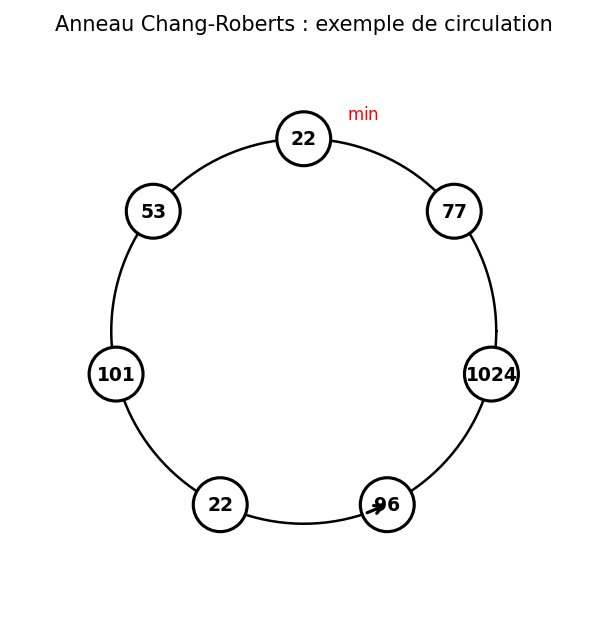
\includegraphics[width=0.52\textwidth]{figures/fig_chang_roberts_ring.png}
  \caption{Anneau orienté à 7 processus — exemple d'exécution de Chang-Roberts.}
  \label{fig:cr_ring}
\end{figure}

% ═══════════════════════════════════════════════════════════
\section{Algorithme de Chang et Roberts (extinction sélective)}
% ═══════════════════════════════════════════════════════════

\begin{definition}[Principe]
  L'élu est le processus possédant le \emph{plus petit identificateur} (entier).
  Le réseau est un anneau orienté ; le protocole est \emph{asynchrone}.
\end{definition}

\paragraph{Idée.}
Lors d'un réveil, un processus ``tente'' de faire parcourir son numéro le tour
de l'anneau. On fait en sorte que seul le plus petit numéro puisse accomplir
ce tour complet.

% ──────────────────────────────────────────
\subsection{Pseudo-code}

Chaque processus dispose :
\begin{itemize}[noitemsep]
  \item d'une \textbf{constante} $\monnum$ (son identifiant unique),
  \item d'une \textbf{variable} $\participant$ (booléen, initialisé à $\mathtt{faux}$),
  \item d'une \textbf{variable} $\leader$ (booléen, initialisé à $\mathtt{faux}$).
\end{itemize}

\medskip
\noindent\textbf{Lors du réveil} (déclenché par la couche supérieure) :
\begin{quote}\ttfamily
si non participant alors\\
\quad envoyer(+, mon\_numero);\\
\quad participant := vrai;
\end{quote}

\medskip
\noindent\textbf{Lors de la réception de $(+, \mathtt{val})$ sur le lien entrant} :
\begin{quote}\ttfamily
si non participant alors\\
\quad participant := vrai;\\
\quad si val < mon\_numero alors envoyer(+, val);\\
\quad sinon envoyer(+, mon\_numero);\\[0.5em]
sinon si val < mon\_numero alors\\
\quad envoyer(+, val);\\
si val = mon\_numero alors\\
\quad leader := vrai;\\
\quad <STOP>\\
// sinon on ne fait rien
\end{quote}

% ──────────────────────────────────────────
\subsection{Preuve de correction}

\subsubsection{Terminaison}

\begin{proof}
Le processus avec le plus petit numéro $p_{\min}$ se réveille nécessairement
à un certain moment.

On raisonne par \emph{induction sur la distance} entre un processus qui se réveille
et $p_{\min}$ : à chaque étape, le message portant $\monnum(p_{\min})$ progresse
d'au moins un saut.

Par induction sur la distance parcourue par le message de $p_{\min}$, ce dernier
fait le tour complet de l'anneau en temps fini.
Lorsque $p_{\min}$ reçoit son propre identifiant, il se déclare leader.
\end{proof}

\subsubsection{Complexité}

\begin{proposition}
  La complexité en nombre de messages est $O(n^2)$.
\end{proposition}

\begin{proof}
La borne supérieure est $n \times n$. Une exécution particulière atteint cette
borne lorsque les processus sont rangés par ordre décroissant de leurs
identifiants (Figure~\ref{fig:worst_case}) : le processus d'identifiant $k$ fait
circuler son message sur $k$ sauts avant d'être éliminé, ce qui donne
$\sum_{k=1}^{n} k = \frac{n(n+1)}{2} = O(n^2)$ messages au total.
\end{proof}

\begin{figure}[H]
  \centering
  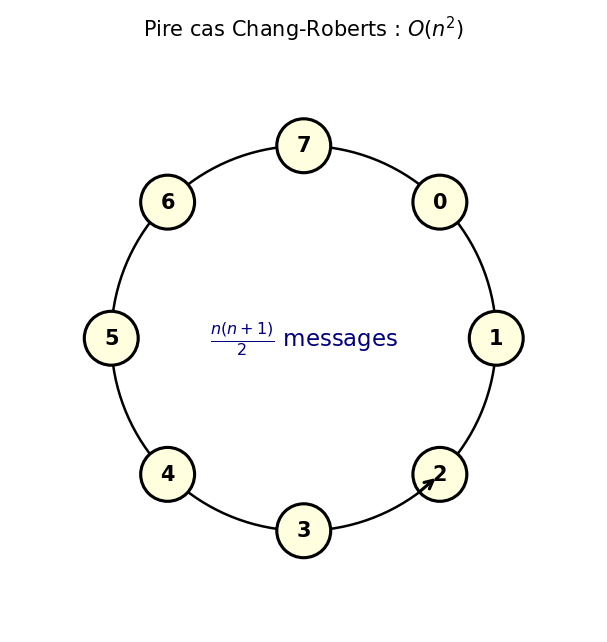
\includegraphics[width=0.50\textwidth]{figures/fig_worst_case_ring.png}
  \caption{Pire cas pour Chang-Roberts : processus rangés par ordre décroissant,
           complexité $O(n^2)$.}
  \label{fig:worst_case}
\end{figure}

% ═══════════════════════════════════════════════════════════
\section{Algorithme de Peterson}
% ═══════════════════════════════════════════════════════════

\begin{definition}[Cadre]
  Anneau \emph{bidirectionnel} (mais orienté).
  Une \textbf{phase} est une unité d'exécution dans laquelle un processus émet
  un message dans un sens et reçoit un message (ou inversement).
  Chaque phase produit des \emph{victimes} et des \emph{survivants}.
\end{definition}

% ──────────────────────────────────────────
\subsection{Idée générale}

\begin{enumerate}[noitemsep]
  \item Une exécution procède par une succession de phases, alternant les
        directions $+$ et $-$.
  \item Une phase est un segment d'exécution dans lequel un processus émet un
        message et reçoit un message, ou vice-versa.
        \begin{remarque}
          Chaque processus a son propre rythme de phase.
        \end{remarque}
  \item Chaque phase fait des victimes et laisse des survivants.
        Une \textbf{victime} est un processus qui reçoit une valeur
        \emph{strictement plus petite} que son propre numéro.
        Par la suite, une victime se contente de relayer les messages.
  \item Lorsqu'un processus survivant termine une phase, il entame la phase
        suivante en envoyant son numéro dans la \emph{direction opposée} à celle
        de la phase précédente.
  \item Un processus qui reçoit son propre numéro devient leader.
\end{enumerate}

\begin{figure}[H]
  \centering
  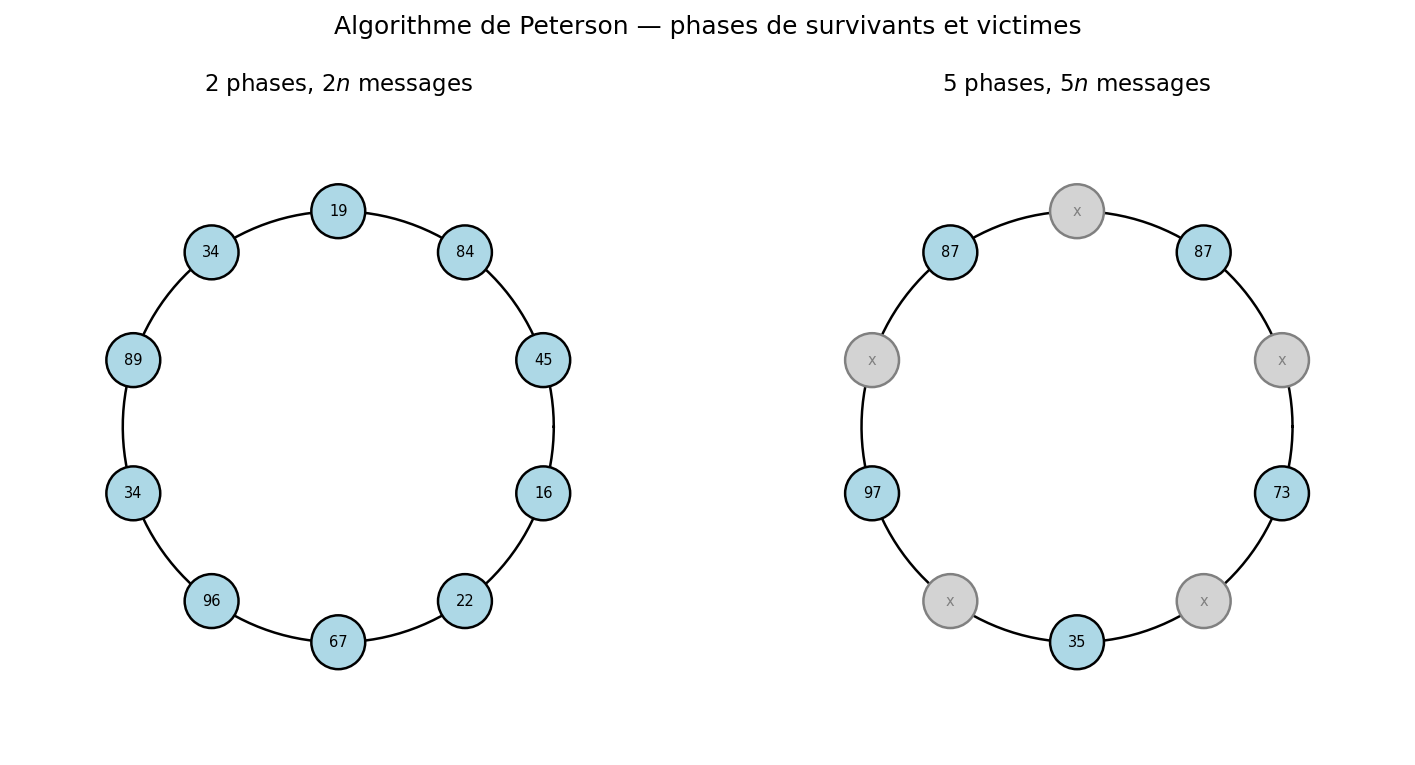
\includegraphics[width=0.85\textwidth]{figures/fig_peterson_phases.png}
  \caption{Algorithme de Peterson : à gauche 2~phases ($2n$~messages),
           à droite 5~phases ($5n$~messages).
           Les nœuds grisés sont les processus morts (victimes).}
  \label{fig:peterson_phases}
\end{figure}

% ──────────────────────────────────────────
\subsection{Éléments de preuve}

\begin{proposition}
  \begin{enumerate}[noitemsep]
    \item Le nombre de phases est fini.
    \item Au bout d'un certain temps, le plus petit numéro fait le tour de l'anneau.
  \end{enumerate}
\end{proposition}

Le point clé est le lemme suivant :

\begin{proposition}[Division par 2]
  Toutes les deux phases, le nombre de processus vivants est divisé par au
  moins~$2$.
  En conséquence, le nombre total de phases est $O(\log n)$, et le nombre total
  de messages est $O(n \log n)$.
\end{proposition}

\begin{proof}
Soit $a$ le numéro d'un processus survivant à la fin de deux phases consécutives
$i$ et $i+1$ (Figure~\ref{fig:peterson_halving}).

\begin{itemize}
  \item Durant la phase $i$, $a$ a reçu une valeur $b$ dans le sens $-$ ;
        comme $a$ est \emph{vivant}, on a $b > a$.
  \item Durant la phase $i+1$, $a$ a reçu une valeur \emph{encore plus grande}.
\end{itemize}

Ainsi $b$ est le plus petit numéro vivant à la fin de la phase $i+1$ dans le
sens $-$ par rapport à $a$.

On construit une \emph{injection} $c \mapsto c'$ entre les processus survivants
à la fin de la paire de phases $(i, i+1)$ et les victimes faites au cours de
ces deux phases.
L'existence de cette injection implique que le nombre de survivants est au plus
la moitié du nombre de processus au début de la paire, soit :
\[
  |\text{survivants à la fin}| \;\leq\; \frac{|\text{vivants au début}|}{2}.
\]
Après $O(\log n)$ paires de phases, il ne reste qu'un seul processus vivant,
qui se déclare leader.
\end{proof}

\begin{figure}[H]
  \centering
  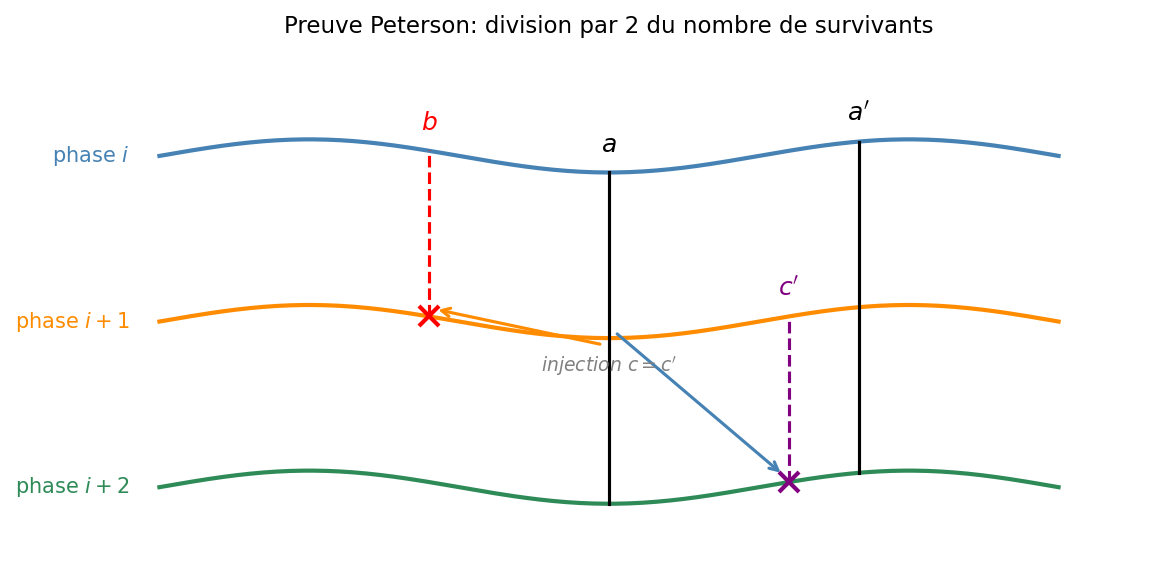
\includegraphics[width=0.82\textwidth]{figures/fig_peterson_halving.png}
  \caption{Diagramme espace-temps illustrant la preuve de division par~2.
           Le processus $a$ survit aux phases $i$ et $i+1$, tandis que $b$ et
           $c'$ sont des victimes.
           L'injection $c = c'$ garantit que le nombre de survivants est divisé
           par~2.}
  \label{fig:peterson_halving}
\end{figure}

\end{document}
